\documentclass{standalone}
\usepackage{tikz}
\usepackage{ctex,siunitx}
\usepackage{tkz-euclide}
\usepackage{amsmath}
\usetikzlibrary{patterns,calc}
\usetikzlibrary {decorations.pathmorphing, decorations.pathreplacing, decorations.shapes,}
\begin{document}
\small
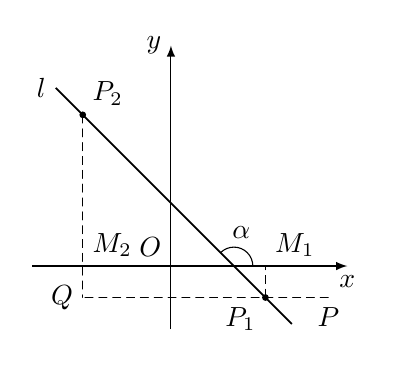
\begin{tikzpicture}[>=latex,scale=0.8]
  \draw[thin,->](-2.2,0)--(2.8,0)node[below]{$x$};
  \draw[thin,->](0,-1.0)--(0,3.5)node[left]{$y$};
  \draw[semithick](1,0)--++(135:4.0)node[left]{$l$};
  \tkzDefPoints{0/0/O,-1.4/2.4/P2,1.5/-0.5/P1,1.5/0/M1,-1.4/0/M2,-1.4/-0.5/Q,2.5/-0.5/P}
  \tkzLabelPoints[above left](O)
  \tkzLabelPoints[left](Q)
  \tkzLabelPoints[below](P)
  \tkzLabelPoint[below left](P1){$P_1$}
  \tkzLabelPoint[above right](P2){$P_2$}
  \tkzLabelPoint[above right](M1){$M_1$}
  \tkzLabelPoint[above right](M2){$M_2$}
  \tkzDrawSegments[densely dashed](P1,M1 P2,Q P,Q)
  \tkzDrawPoints[fill=black](P1,P2)
  \draw[semithick](1,0)--++(-45:1.3);
  \draw(1.3,0)arc(0:135:0.3)node[midway,above]{$\alpha$};
\end{tikzpicture}
\end{document}